\documentclass{minimal}

% Tikz
\usepackage{pgf}
\usepackage{tikz}

\begin{document}

\begin{center}
 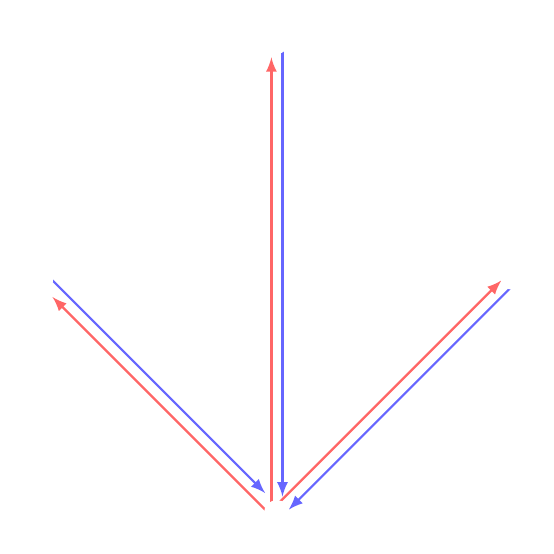
\begin{tikzpicture}
 [
 	vertex/.style={draw=none,circle,fill=white,minimum size=2pt},
 	vertex/.style={draw=none,circle,fill=white,minimum size=2pt},
	oedge/.style={->,>=latex,shorten >=6pt,draw,white,thick},
	roedge/.style={->,>=latex,shorten >=6pt,draw,thick,color=red!60!white},
	boedge/.style={->,>=latex,shorten >=6pt,draw,thick,color=blue!60!white}
 ]

\coordinate (V1) at (-3,3);
\coordinate (V2) at (0,0);
\coordinate (V3) at (0,6);
\coordinate (V4) at (3,3);

\path[boedge] ([yshift=3pt]V1) to ([yshift=3pt]V2) {};
\path[roedge] ([yshift=-3pt]V2) to ([yshift=-3pt]V1) {};

\path[oedge] ([yshift=3pt]V1) -- ([yshift=3pt]V3) {};
\path[oedge] ([yshift=-3pt]V3) -- ([yshift=-3pt]V1) {};

\path[boedge] ([xshift=2pt]V3) -- ([xshift=2pt]V2) {};
\path[roedge] ([xshift=-2pt]V2) -- ([xshift=-2pt]V3) {};

\path[roedge] ([yshift=3pt]V2) -- ([yshift=3pt]V4) {};
\path[boedge] ([yshift=-3pt]V4) -- ([yshift=-3pt]V2) {};

\path[oedge] ([yshift=3pt]V3) -- ([yshift=3pt]V4) {};
\path[oedge] ([yshift=-3pt]V4) -- ([yshift=-3pt]V3) {};

\node[vertex] at (V1) {};
\node[vertex] at (V2) {};
\node[vertex] at (V3) {};
\node[vertex] at (V4) {};

%\draw[->, thick] (-0.4,3) arc (0:320:20pt);


\end{tikzpicture}
\end{center}

\end{document}
